% Options for packages loaded elsewhere
\PassOptionsToPackage{unicode}{hyperref}
\PassOptionsToPackage{hyphens}{url}
%
\documentclass[
  doc]{apa6}
\usepackage{amsmath,amssymb}
\usepackage{lmodern}
\usepackage{iftex}
\ifPDFTeX
  \usepackage[T1]{fontenc}
  \usepackage[utf8]{inputenc}
  \usepackage{textcomp} % provide euro and other symbols
\else % if luatex or xetex
  \usepackage{unicode-math}
  \defaultfontfeatures{Scale=MatchLowercase}
  \defaultfontfeatures[\rmfamily]{Ligatures=TeX,Scale=1}
\fi
% Use upquote if available, for straight quotes in verbatim environments
\IfFileExists{upquote.sty}{\usepackage{upquote}}{}
\IfFileExists{microtype.sty}{% use microtype if available
  \usepackage[]{microtype}
  \UseMicrotypeSet[protrusion]{basicmath} % disable protrusion for tt fonts
}{}
\makeatletter
\@ifundefined{KOMAClassName}{% if non-KOMA class
  \IfFileExists{parskip.sty}{%
    \usepackage{parskip}
  }{% else
    \setlength{\parindent}{0pt}
    \setlength{\parskip}{6pt plus 2pt minus 1pt}}
}{% if KOMA class
  \KOMAoptions{parskip=half}}
\makeatother
\usepackage{xcolor}
\IfFileExists{xurl.sty}{\usepackage{xurl}}{} % add URL line breaks if available
\IfFileExists{bookmark.sty}{\usepackage{bookmark}}{\usepackage{hyperref}}
\hypersetup{
  pdftitle={Do owners know how impulsive their dogs are?},
  pdfauthor={Jeffrey R. Stevens1, Madeline Mathias1, Megan Herridge1, Kylie Hughes-Duvall1, London M. Wolff1, \& McKenna Yohe1},
  pdflang={en-EN},
  hidelinks,
  pdfcreator={LaTeX via pandoc}}
\urlstyle{same} % disable monospaced font for URLs
\usepackage{graphicx}
\makeatletter
\def\maxwidth{\ifdim\Gin@nat@width>\linewidth\linewidth\else\Gin@nat@width\fi}
\def\maxheight{\ifdim\Gin@nat@height>\textheight\textheight\else\Gin@nat@height\fi}
\makeatother
% Scale images if necessary, so that they will not overflow the page
% margins by default, and it is still possible to overwrite the defaults
% using explicit options in \includegraphics[width, height, ...]{}
\setkeys{Gin}{width=\maxwidth,height=\maxheight,keepaspectratio}
% Set default figure placement to htbp
\makeatletter
\def\fps@figure{htbp}
\makeatother
\setlength{\emergencystretch}{3em} % prevent overfull lines
\providecommand{\tightlist}{%
  \setlength{\itemsep}{0pt}\setlength{\parskip}{0pt}}
\setcounter{secnumdepth}{-\maxdimen} % remove section numbering
% Make \paragraph and \subparagraph free-standing
\ifx\paragraph\undefined\else
  \let\oldparagraph\paragraph
  \renewcommand{\paragraph}[1]{\oldparagraph{#1}\mbox{}}
\fi
\ifx\subparagraph\undefined\else
  \let\oldsubparagraph\subparagraph
  \renewcommand{\subparagraph}[1]{\oldsubparagraph{#1}\mbox{}}
\fi
\ifLuaTeX
\usepackage[bidi=basic]{babel}
\else
\usepackage[bidi=default]{babel}
\fi
\babelprovide[main,import]{english}
% get rid of language-specific shorthands (see #6817):
\let\LanguageShortHands\languageshorthands
\def\languageshorthands#1{}
% Manuscript styling
\usepackage{upgreek}
\captionsetup{font=singlespacing,justification=justified}

% Table formatting
\usepackage{longtable}
\usepackage{lscape}
% \usepackage[counterclockwise]{rotating}   % Landscape page setup for large tables
\usepackage{multirow}		% Table styling
\usepackage{tabularx}		% Control Column width
\usepackage[flushleft]{threeparttable}	% Allows for three part tables with a specified notes section
\usepackage{threeparttablex}            % Lets threeparttable work with longtable

% Create new environments so endfloat can handle them
% \newenvironment{ltable}
%   {\begin{landscape}\centering\begin{threeparttable}}
%   {\end{threeparttable}\end{landscape}}
\newenvironment{lltable}{\begin{landscape}\centering\begin{ThreePartTable}}{\end{ThreePartTable}\end{landscape}}

% Enables adjusting longtable caption width to table width
% Solution found at http://golatex.de/longtable-mit-caption-so-breit-wie-die-tabelle-t15767.html
\makeatletter
\newcommand\LastLTentrywidth{1em}
\newlength\longtablewidth
\setlength{\longtablewidth}{1in}
\newcommand{\getlongtablewidth}{\begingroup \ifcsname LT@\roman{LT@tables}\endcsname \global\longtablewidth=0pt \renewcommand{\LT@entry}[2]{\global\advance\longtablewidth by ##2\relax\gdef\LastLTentrywidth{##2}}\@nameuse{LT@\roman{LT@tables}} \fi \endgroup}

% \setlength{\parindent}{0.5in}
% \setlength{\parskip}{0pt plus 0pt minus 0pt}

% Overwrite redefinition of paragraph and subparagraph by the default LaTeX template
% See https://github.com/crsh/papaja/issues/292
\makeatletter
\renewcommand{\paragraph}{\@startsection{paragraph}{4}{\parindent}%
  {0\baselineskip \@plus 0.2ex \@minus 0.2ex}%
  {-1em}%
  {\normalfont\normalsize\bfseries\itshape\typesectitle}}

\renewcommand{\subparagraph}[1]{\@startsection{subparagraph}{5}{1em}%
  {0\baselineskip \@plus 0.2ex \@minus 0.2ex}%
  {-\z@\relax}%
  {\normalfont\normalsize\itshape\hspace{\parindent}{#1}\textit{\addperi}}{\relax}}
\makeatother

% \usepackage{etoolbox}
\makeatletter
\patchcmd{\HyOrg@maketitle}
  {\section{\normalfont\normalsize\abstractname}}
  {\section*{\normalfont\normalsize\abstractname}}
  {}{\typeout{Failed to patch abstract.}}
\patchcmd{\HyOrg@maketitle}
  {\section{\protect\normalfont{\@title}}}
  {\section*{\protect\normalfont{\@title}}}
  {}{\typeout{Failed to patch title.}}
\makeatother

\usepackage{xpatch}
\makeatletter
\xapptocmd\appendix
  {\xapptocmd\section
    {\addcontentsline{toc}{section}{\appendixname\ifoneappendix\else~\theappendix\fi\\: #1}}
    {}{\InnerPatchFailed}%
  }
{}{\PatchFailed}
\usepackage{csquotes}
\ifLuaTeX
  \usepackage{selnolig}  % disable illegal ligatures
\fi

\title{Do owners know how impulsive their dogs are?}
\author{Jeffrey R. Stevens\textsuperscript{1}, Madeline Mathias\textsuperscript{1}, Megan Herridge\textsuperscript{1}, Kylie Hughes-Duvall\textsuperscript{1}, London M. Wolff\textsuperscript{1}, \& McKenna Yohe\textsuperscript{1}}
\date{}


\shorttitle{Do owners know how impulsive their dogs are?}

\authornote{

Correspondence concerning this article should be addressed to Jeffrey R. Stevens, B83 East Stadium, University of Nebraska, Lincoln, Lincoln, NE, USA 68588. ORCID 0000-0003-2375-1360. E-mail: \href{mailto:jeffrey.r.stevens@gmail.com}{\nolinkurl{jeffrey.r.stevens@gmail.com}}

}

\affiliation{\vspace{0.5cm}\textsuperscript{1} University of Nebraska-Lincoln}

\begin{document}
\maketitle

\renewcommand{\thetable}{S\arabic{table}}
\setcounter{table}{0}
\renewcommand{\thefigure}{S\arabic{figure}}
\setcounter{figure}{0}
\setcounter{page}{1}

\begin{table}[!h]

\caption{\label{tab:demographics}Dog owner demographic information}
\centering
\begin{threeparttable}
\begin{tabular}[t]{lrr}
\toprule
 & Study 1 (N=65) & Study 2 (N=43)\\
\addlinespace[0.3em]
\multicolumn{3}{l}{\textbf{Gender}}\\
\hspace{1em}Female & 49 (76.6\%) & 39 (90.7\%)\\
\hspace{1em}Male & 15 (23.4\%) & 4 (9.3\%)\\
\hspace{1em}Nonbinary & 0 (0\%) & 0 (0\%)\\
\addlinespace[0.3em]
\multicolumn{3}{l}{\textbf{Marital status}}\\
\hspace{1em}Single & 20 (31.2\%) & 18 (41.9\%)\\
\hspace{1em}Married & 40 (62.5\%) & 22 (51.2\%)\\
\hspace{1em}Separated/divorced & 4 (6.2\%) & 2 (4.7\%)\\
\hspace{1em}Widowed & 0 (0\%) & 1 (2.3\%)\\
\addlinespace[0.3em]
\multicolumn{3}{l}{\textbf{Have other dogs}}\\
\hspace{1em}Yes & 34 (53.1\%) & 21 (48.8\%)\\
\hspace{1em}No & 30 (46.9\%) & 22 (51.2\%)\\
\addlinespace[0.3em]
\multicolumn{3}{l}{\textbf{Household income}}\\
\hspace{1em}<\$25,000 & 6 (9.5\%) & 9 (20.9\%)\\
\hspace{1em}\$25,001-\$50,000 & 11 (17.5\%) & 5 (11.6\%)\\
\hspace{1em}\$50,001-\$75,000 & 8 (12.7\%) & 7 (16.3\%)\\
\hspace{1em}\$75,001-\$100,000 & 16 (25.4\%) & 2 (4.7\%)\\
\hspace{1em}>\$100,000 & 19 (30.2\%) & 14 (32.6\%)\\
\hspace{1em}Prefer not to answer & 3 (4.8\%) & 6 (14.0\%)\\
\bottomrule
\end{tabular}
\begin{tablenotes}
\item \textit{Note: } 
\item Table used with permission under a CC-BY4.0 license: Stevens et al. (2022); available at https://doi.org/10.31234/osf.io/hyvdq.
\end{tablenotes}
\end{threeparttable}
\end{table}

\begin{table}[!h]

\caption{\label{tab:reliability}Scale reliability values}
\centering
\begin{threeparttable}
\begin{tabular}[t]{lrr}
\toprule
Scale & Study 1 & Study 2\\
\midrule
Bennett and Rohlf disobedience & 0.85 & --\\
Bennett and Rohlf aggression & 0.89 & --\\
Bennett and Rohlf nervousness & 0.90 & --\\
Bennett and Rohlf destructiveness & 0.57 & --\\
Bennett and Rohlf excitability & 0.35 & --\\
Hiby et al. obedience & 0.79 & 0.77\\
Hiby et al. problem behaviors & 0.74 & --\\
DIAS overall & 0.86 & 0.83\\
DIAS behavioral regulation & 0.85 & 0.83\\
DIAS aggression & 0.68 & 0.72\\
DIAS responsiveness & 0.59 & 0.46\\
MDORS & 0.71 & --\\
Owner extraversion* & 0.80 & 0.69\\
Owner agreeableness* & 0.31 & 0.54\\
Owner conscientiousness* & 0.45 & 0.37\\
Owner stability* & 0.65 & 0.70\\
Owner openness* & 0.24 & 0.36\\
Cognitive reflection task & 0.59 & --\\
Berlin numeracy test & 0.48 & --\\
CBARQ training & -- & 0.77\\
\bottomrule
\end{tabular}
\begin{tablenotes}
\item \newline\textit{Note: }  Values represent Revelle's $\omega_{T}$ except owner personality scales (signaled with *), which use Cronbach's $\alpha$. Table used with permission under a CC-BY4.0 license: Stevens et al. (2022); available at https://doi.org/10.31234/osf.io/hyvdq.
\end{tablenotes}
\end{threeparttable}
\end{table}

\clearpage

\begin{figure*}

{\centering 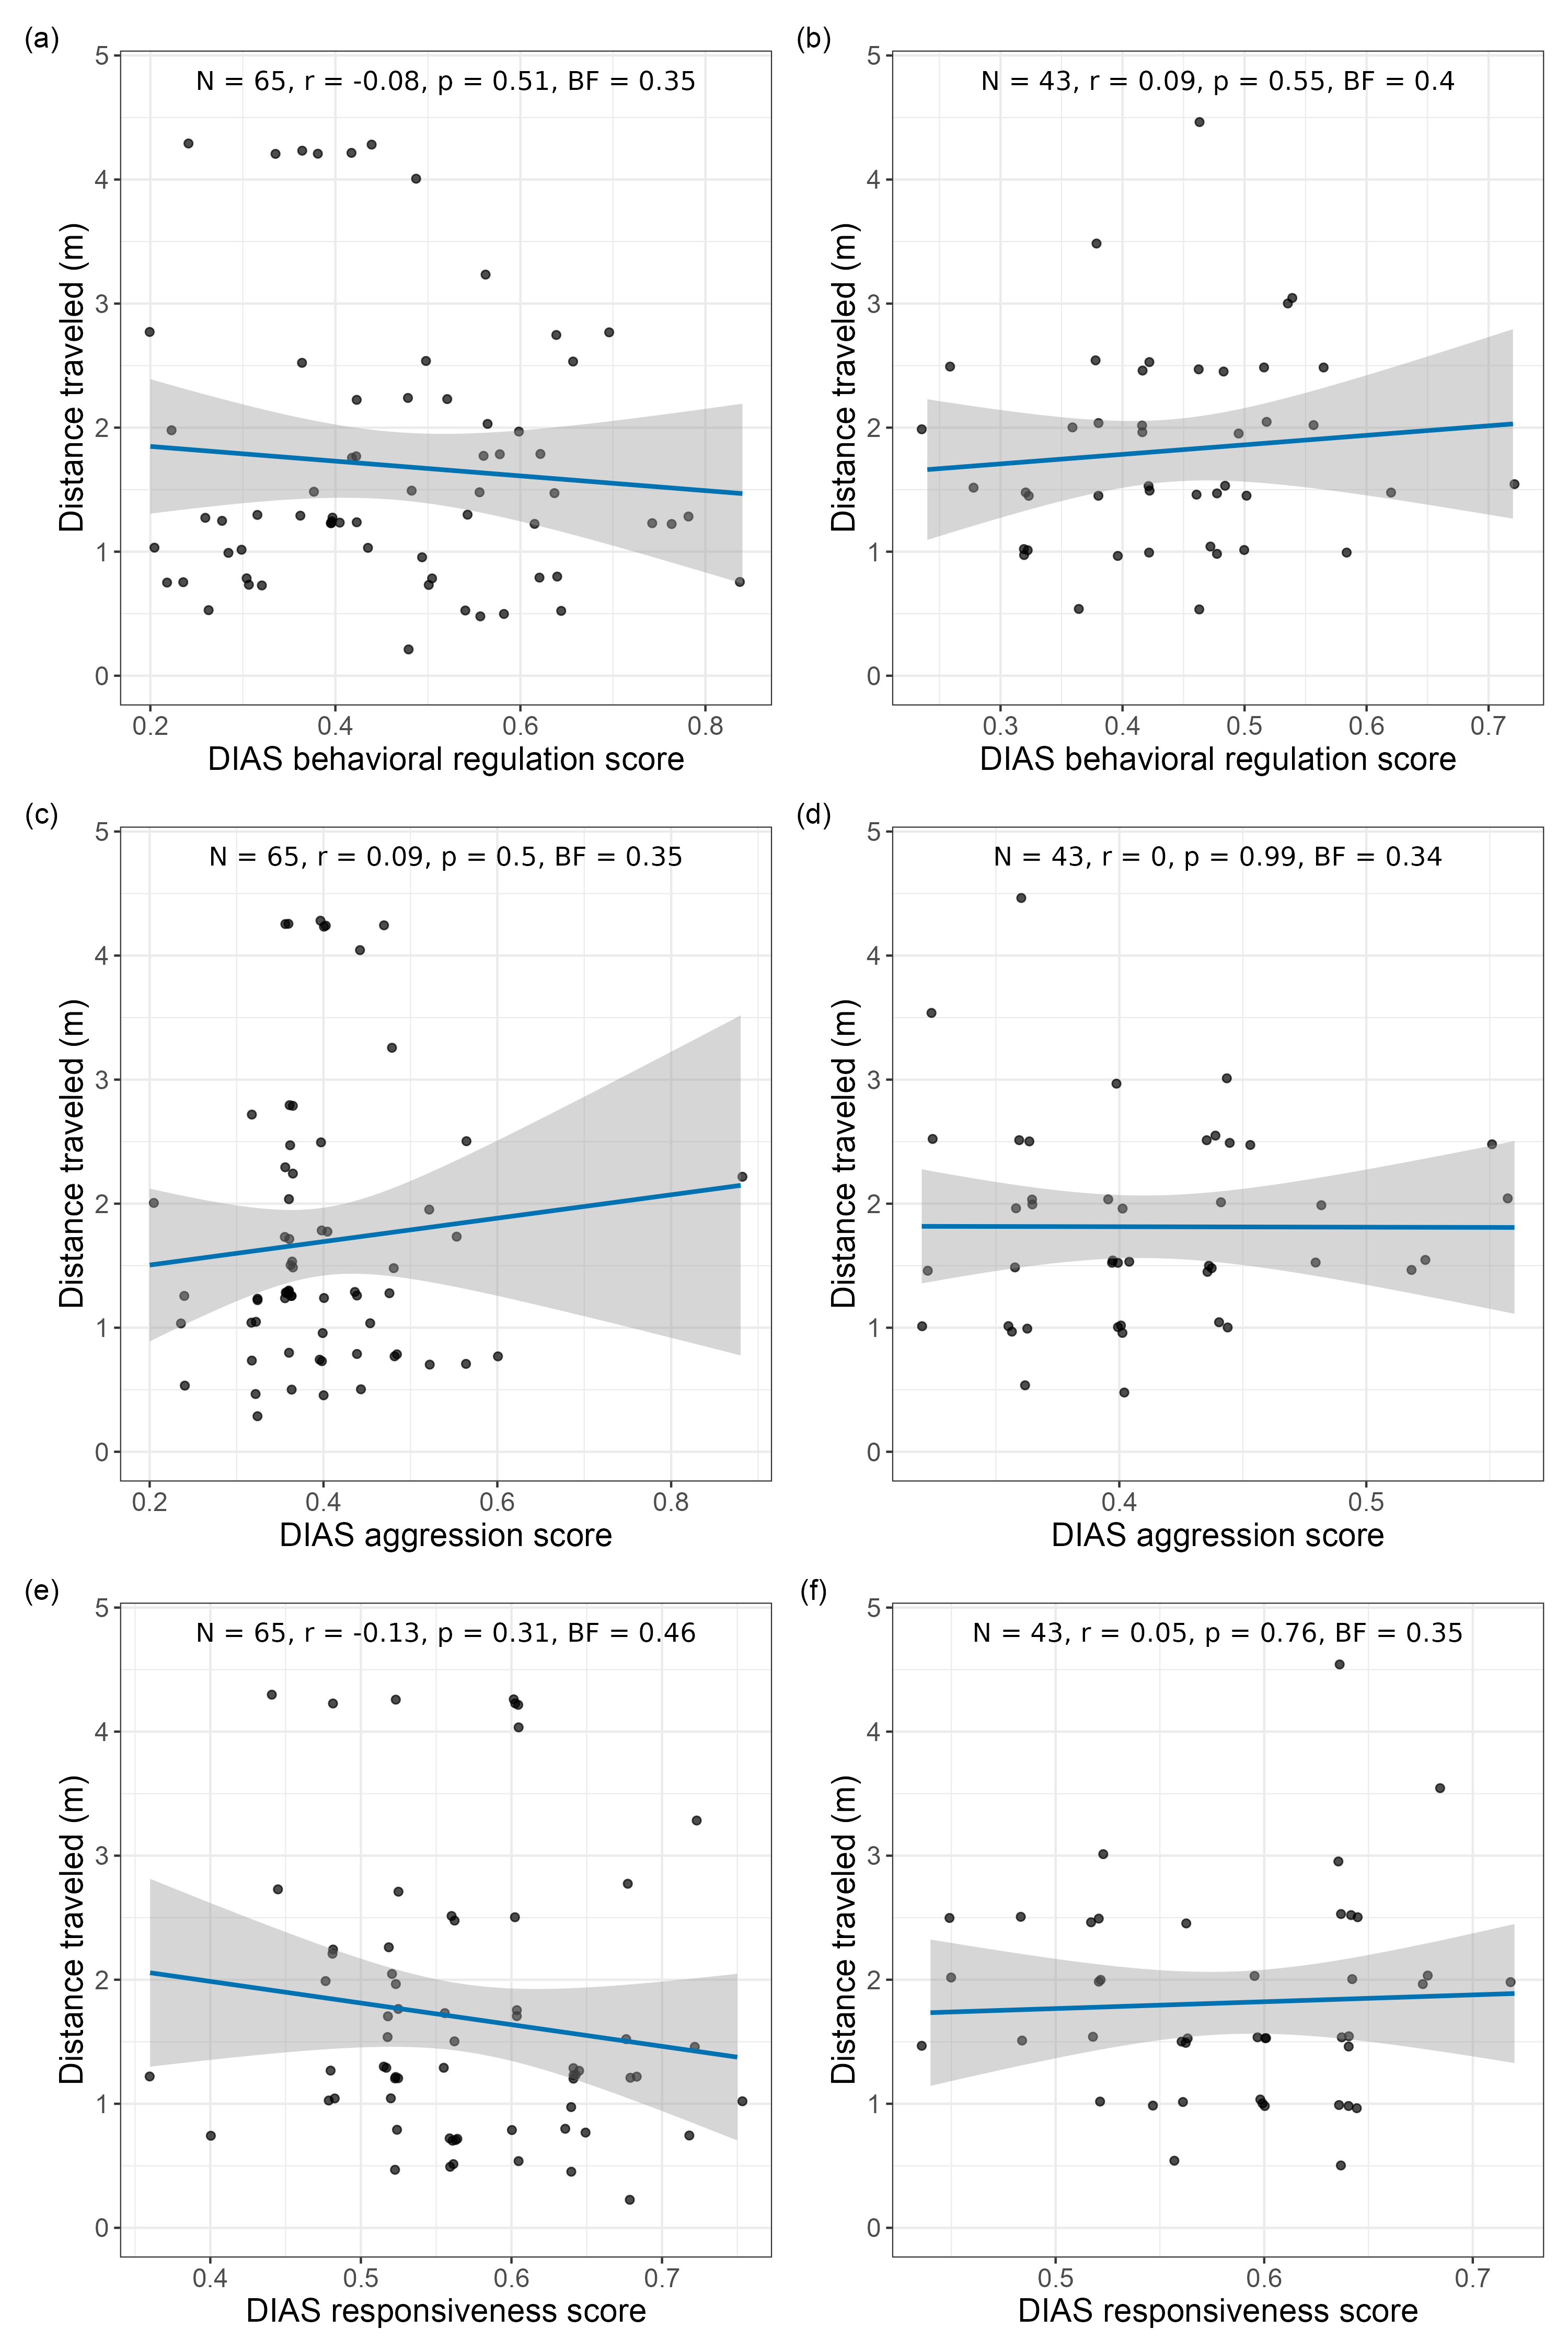
\includegraphics[width=0.75\linewidth]{figures/distance_dias_subscales} 

}

\caption{Relationship between distance traveled and DIAS subscales. We found no correlation between distance traveled and the behavioral regulation subscale in (a) Study 1 or (b) Study 2 or the aggression subscale in (c) Study 1 or (d) Study 2, or the responsiveness subscale in (e) Study 1 or (f) Study 2. Dots represent individual dog data points, lines represent best fitting linear regression models, and bands represent 95\% confidence intervals around the regression models.  Figure used with permission under a CC-BY4.0 license: Stevens et al. (2022); available at https://doi.org/10.31234/osf.io/hyvdq.}\label{fig:dias-all}
\end{figure*}

\begin{figure*}

{\centering 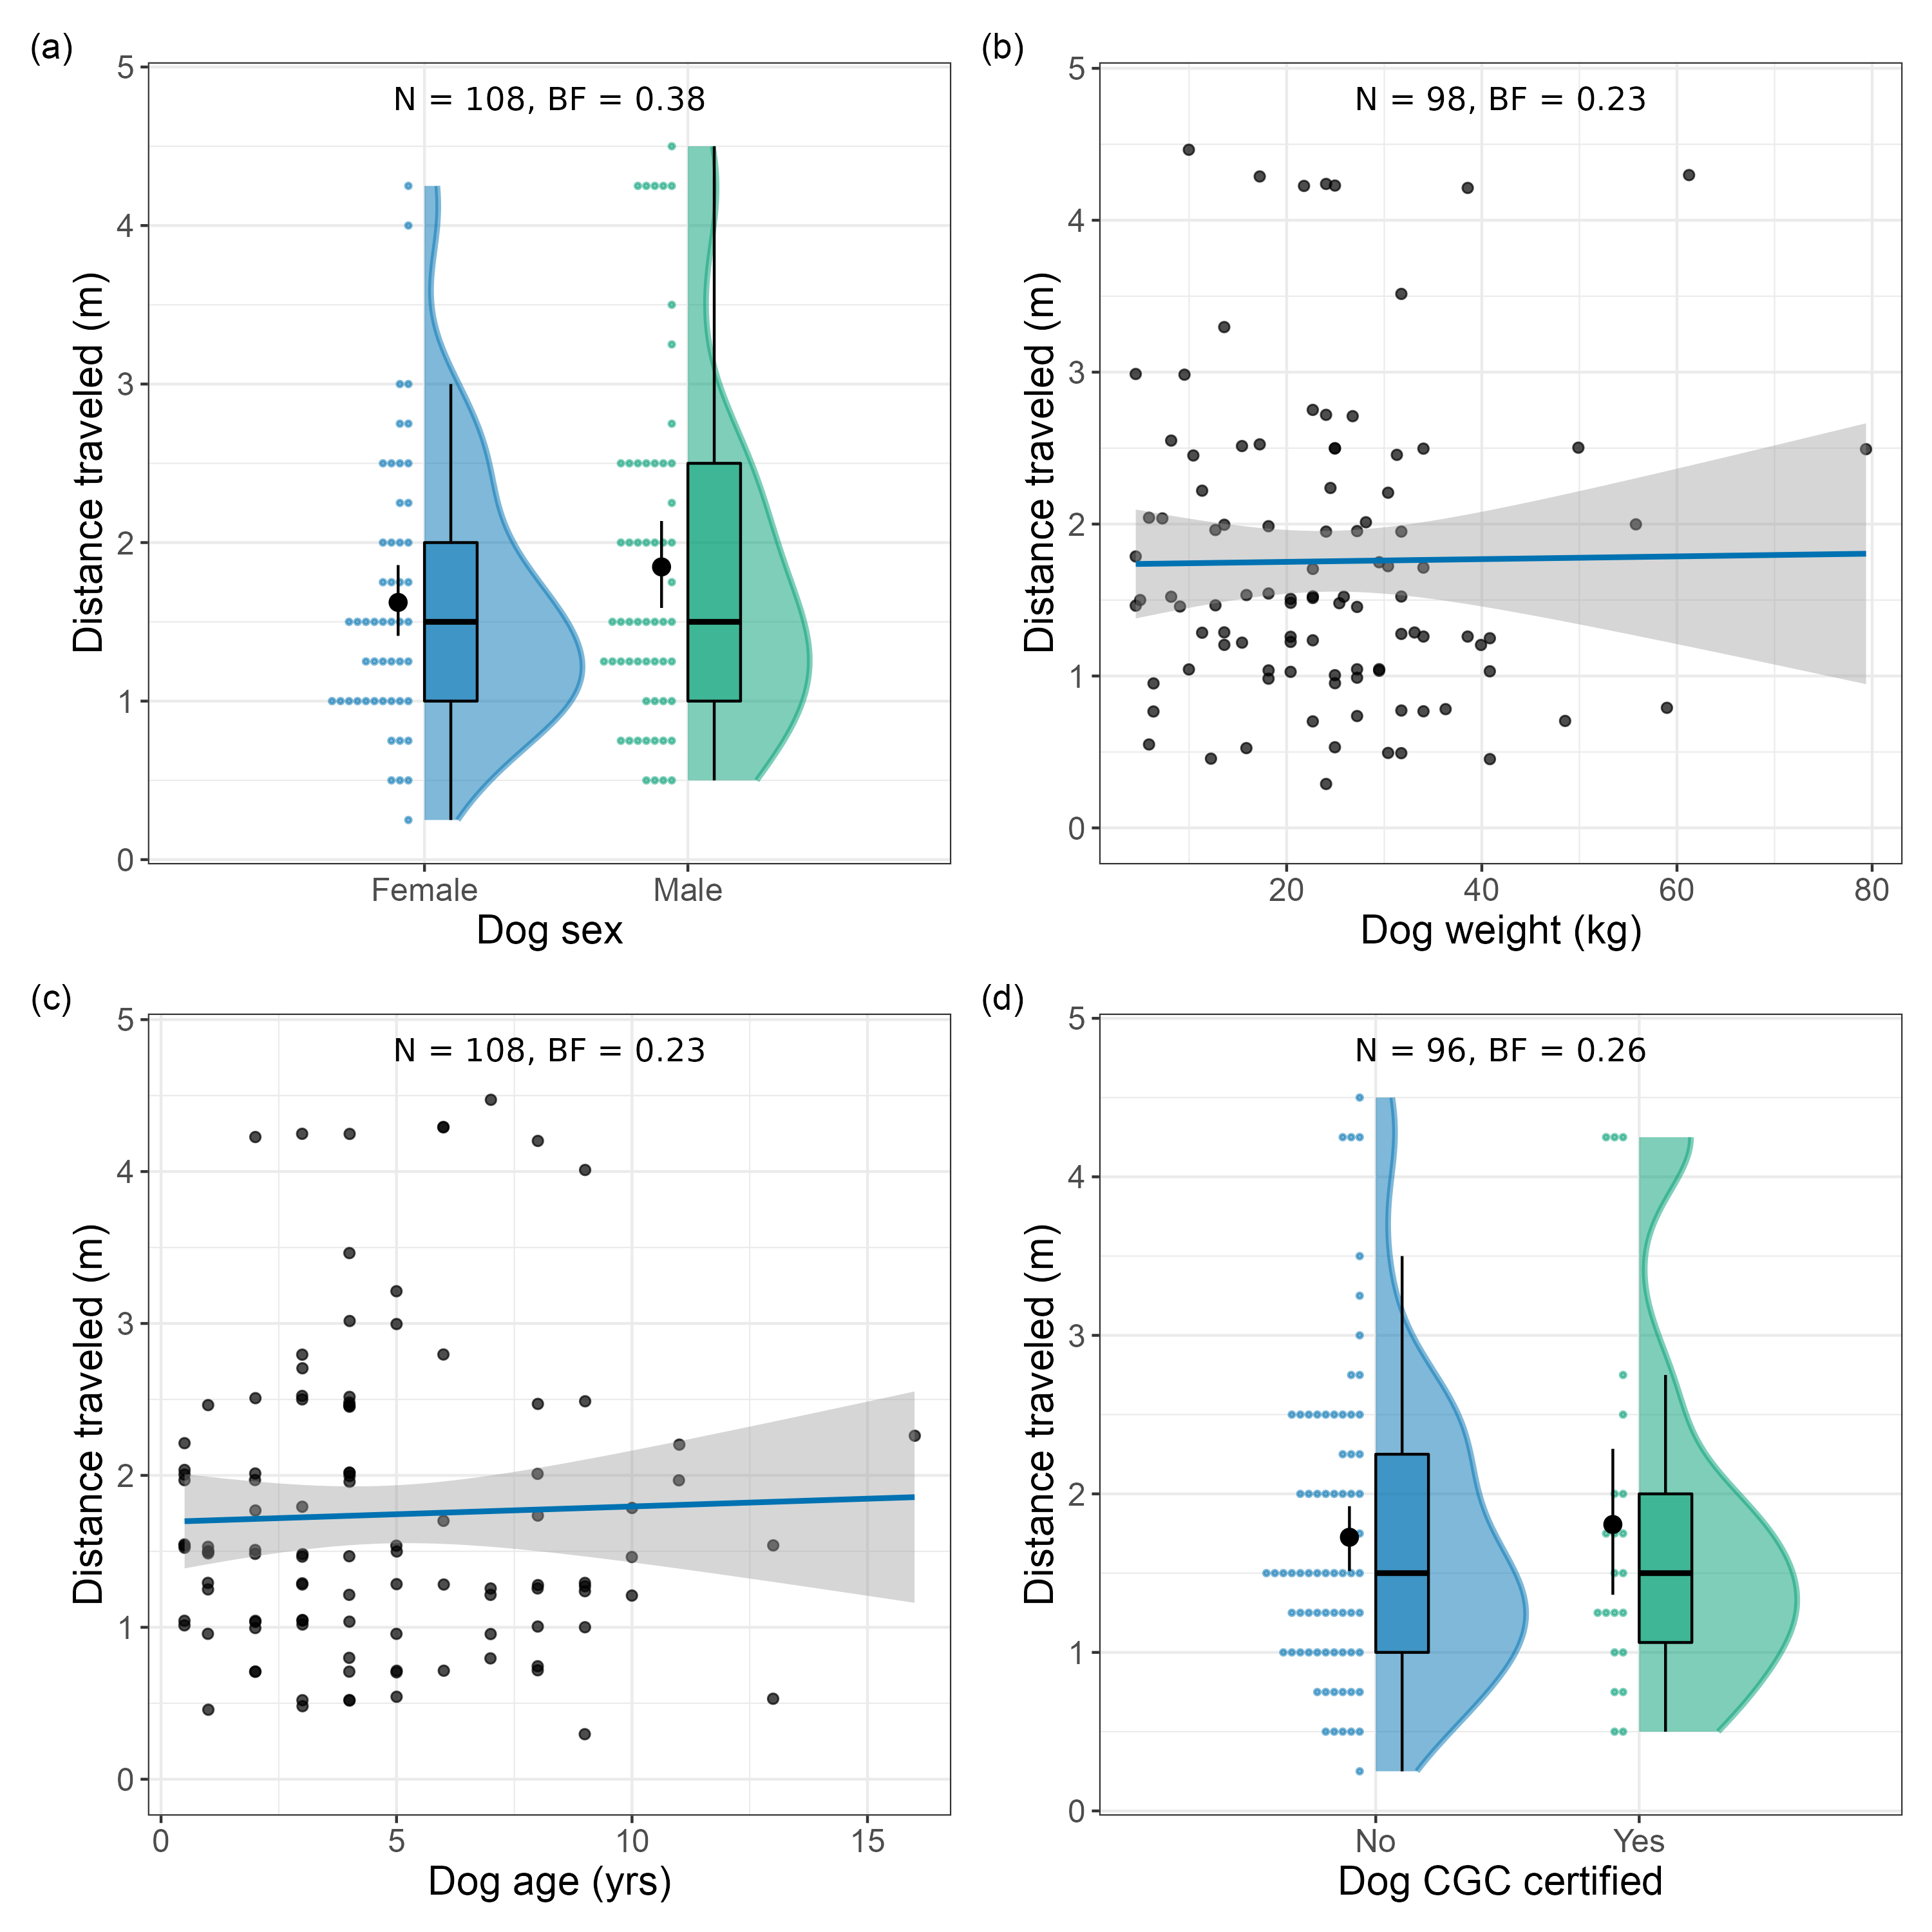
\includegraphics[width=0.95\linewidth]{figures/dog_characteristics} 

}

\caption{Relationship between distance traveled and dog characteristics. Distance traveled was not related to dog (a) sex, (b) weight, (c) age, or (d) AKC Canine Good Citizen status. For correlations, dots represent individual dog data points, lines represent best fitting linear regression models, and bands represent 95\% confidence intervals around the regression models. For group comparisons, dots represent individual dog data points, filled shapes represent density distributions, filled dots and error bars represent means and 95\% confidence intervals, boxes represent interquartile ranges, lines within boxes represent medians, and whiskers represent 1.5 times the interquartile range.  Figure used with permission under a CC-BY4.0 license: Stevens et al. (2022); available at https://doi.org/10.31234/osf.io/hyvdq.}\label{fig:dog-char}
\end{figure*}

\begin{figure*}

{\centering 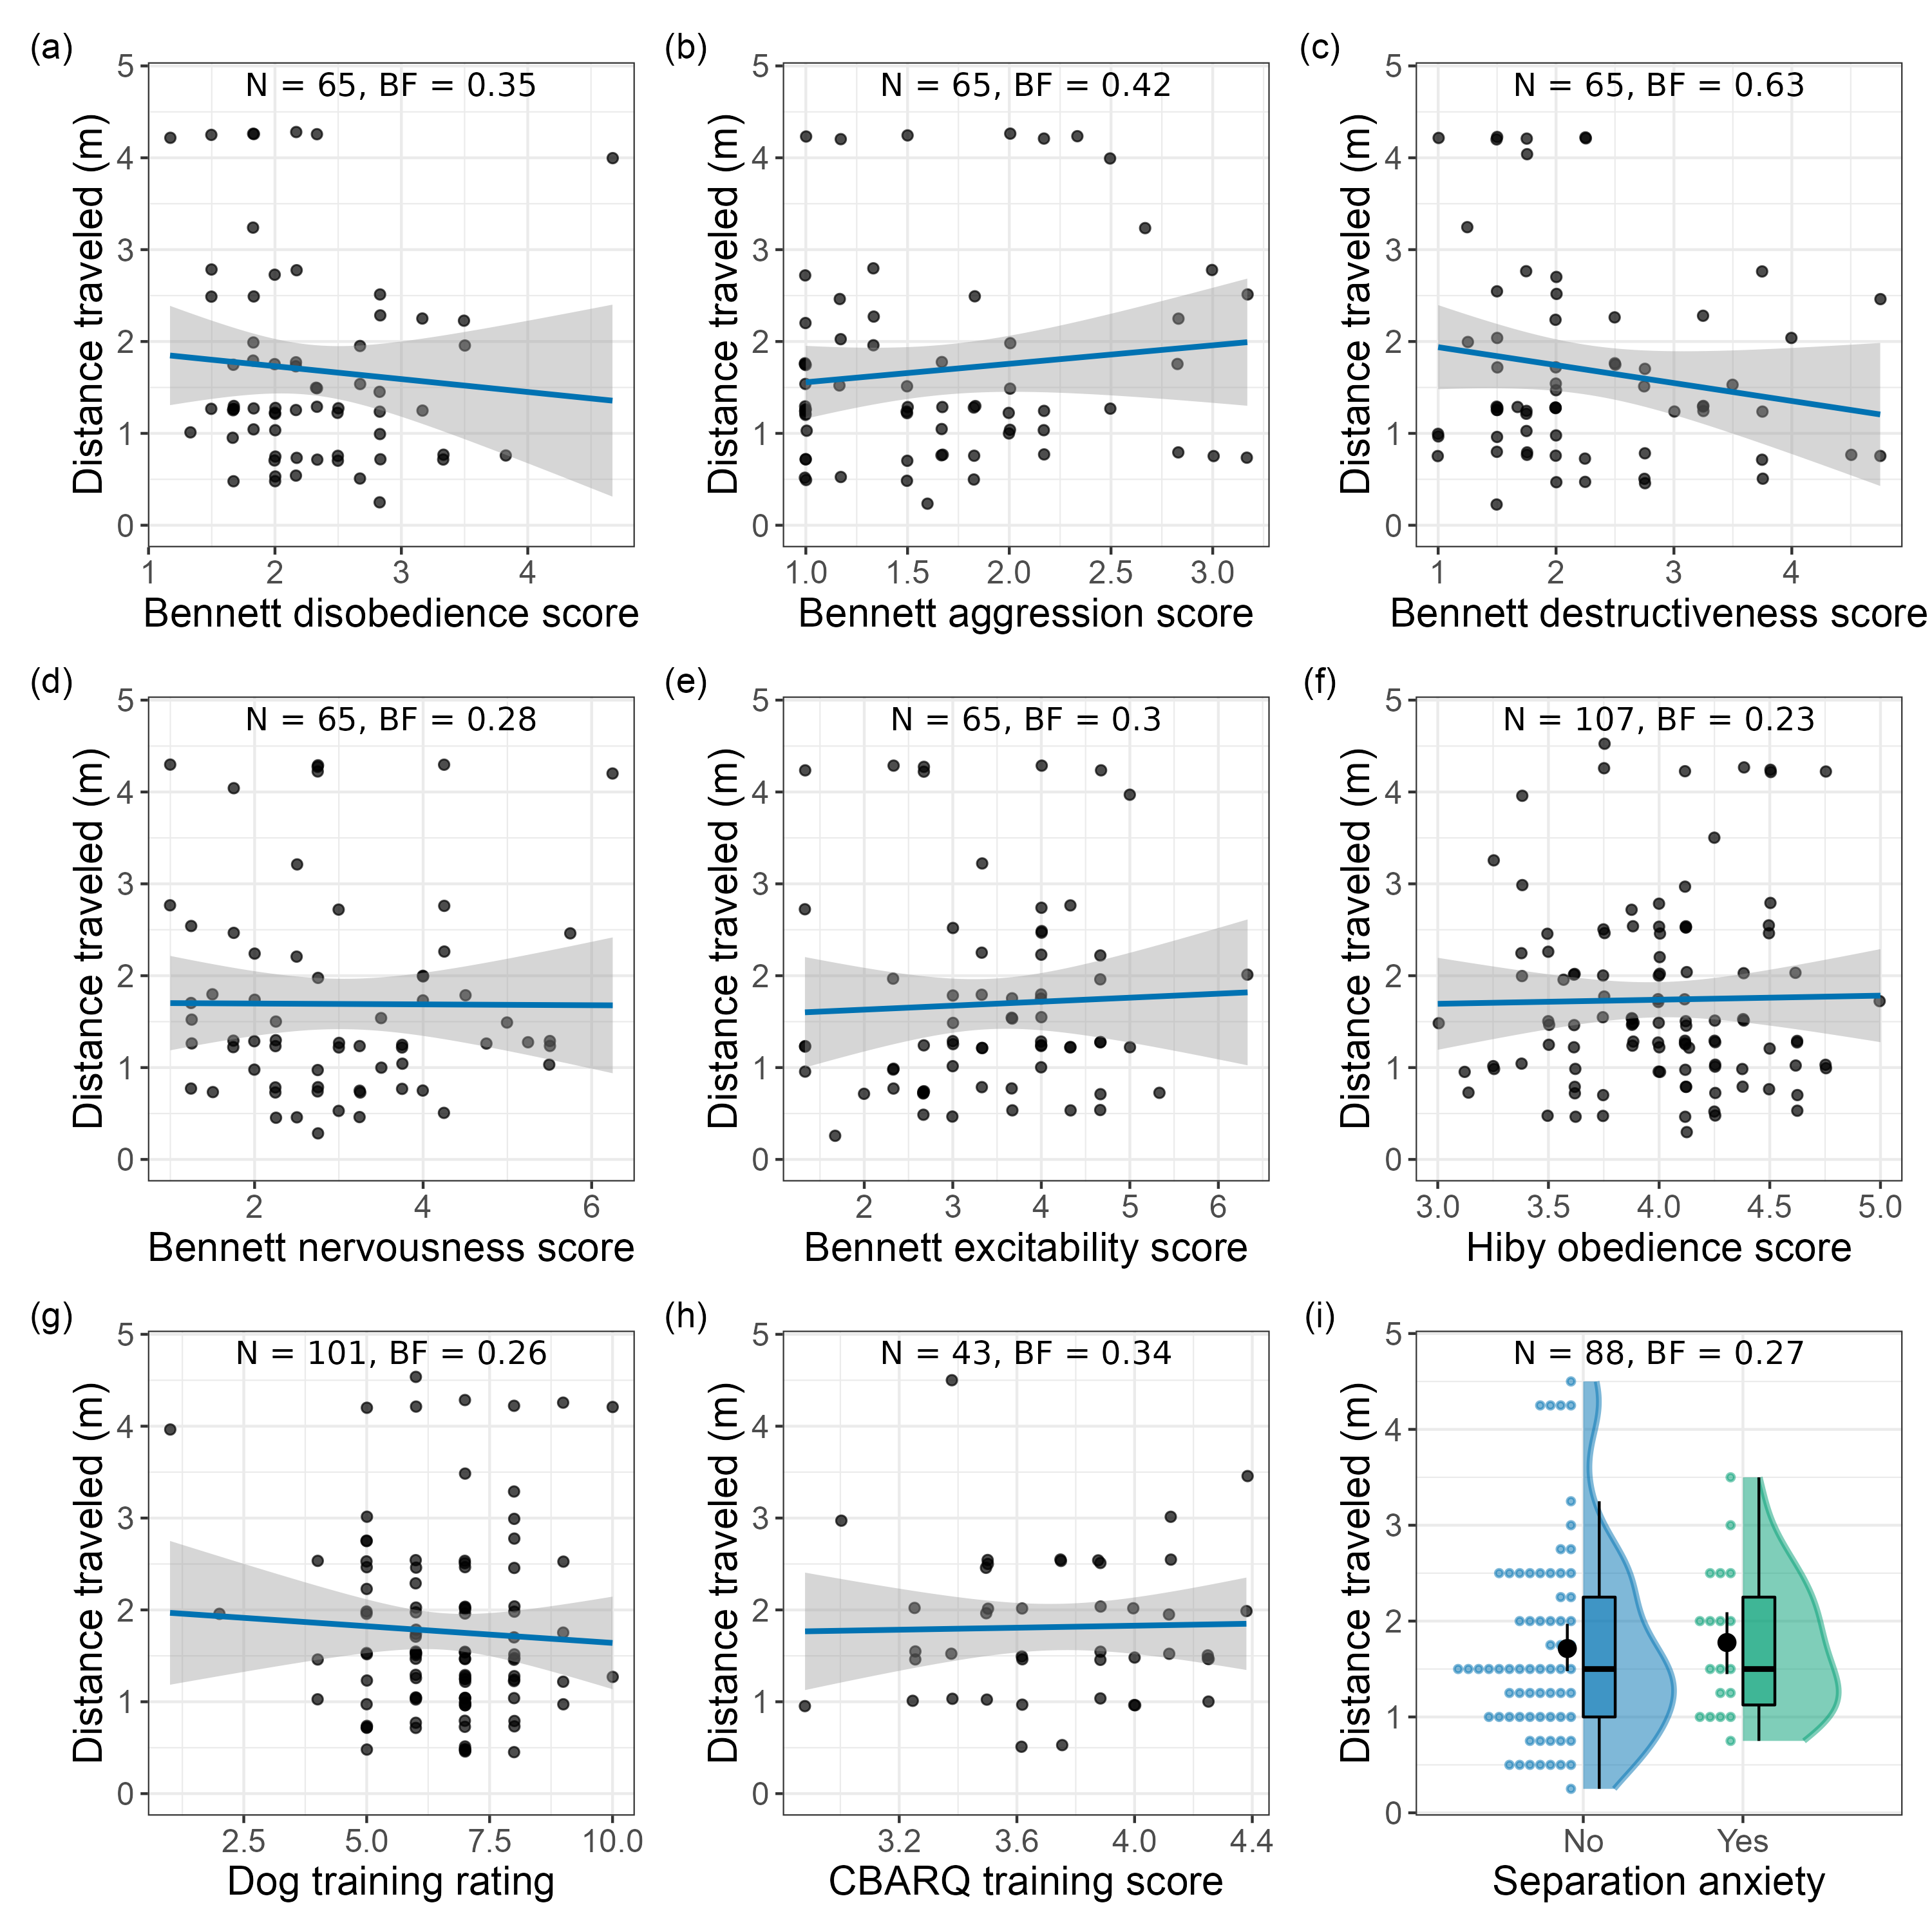
\includegraphics[width=0.95\linewidth]{figures/dog_behavior} 

}

\caption{Relationship between distance traveled and dog behavior. Distance traveled was not related to (a-e) scores on Bennett and Rolhf's (2007) behavior problems scales, (f) Hiby et al.'s (2004) obedience scale, (g-h) measures of training, or (i) ratings of separation anxiety. For correlations, dots represent individual dog data points, lines represent best fitting linear regression models, and bands represent 95\% confidence intervals around the regression models. For group comparisons, dots represent individual dog data points, filled shapes represent density distributions, filled dots and error bars represent means and 95\% confidence intervals, boxes represent interquartile ranges, lines within boxes represent medians, and whiskers represent 1.5 times the interquartile range.  Figure used with permission under a CC-BY4.0 license: Stevens et al. (2022); available at https://doi.org/10.31234/osf.io/hyvdq.}\label{fig:dog-behavior}
\end{figure*}

\begin{figure*}

{\centering 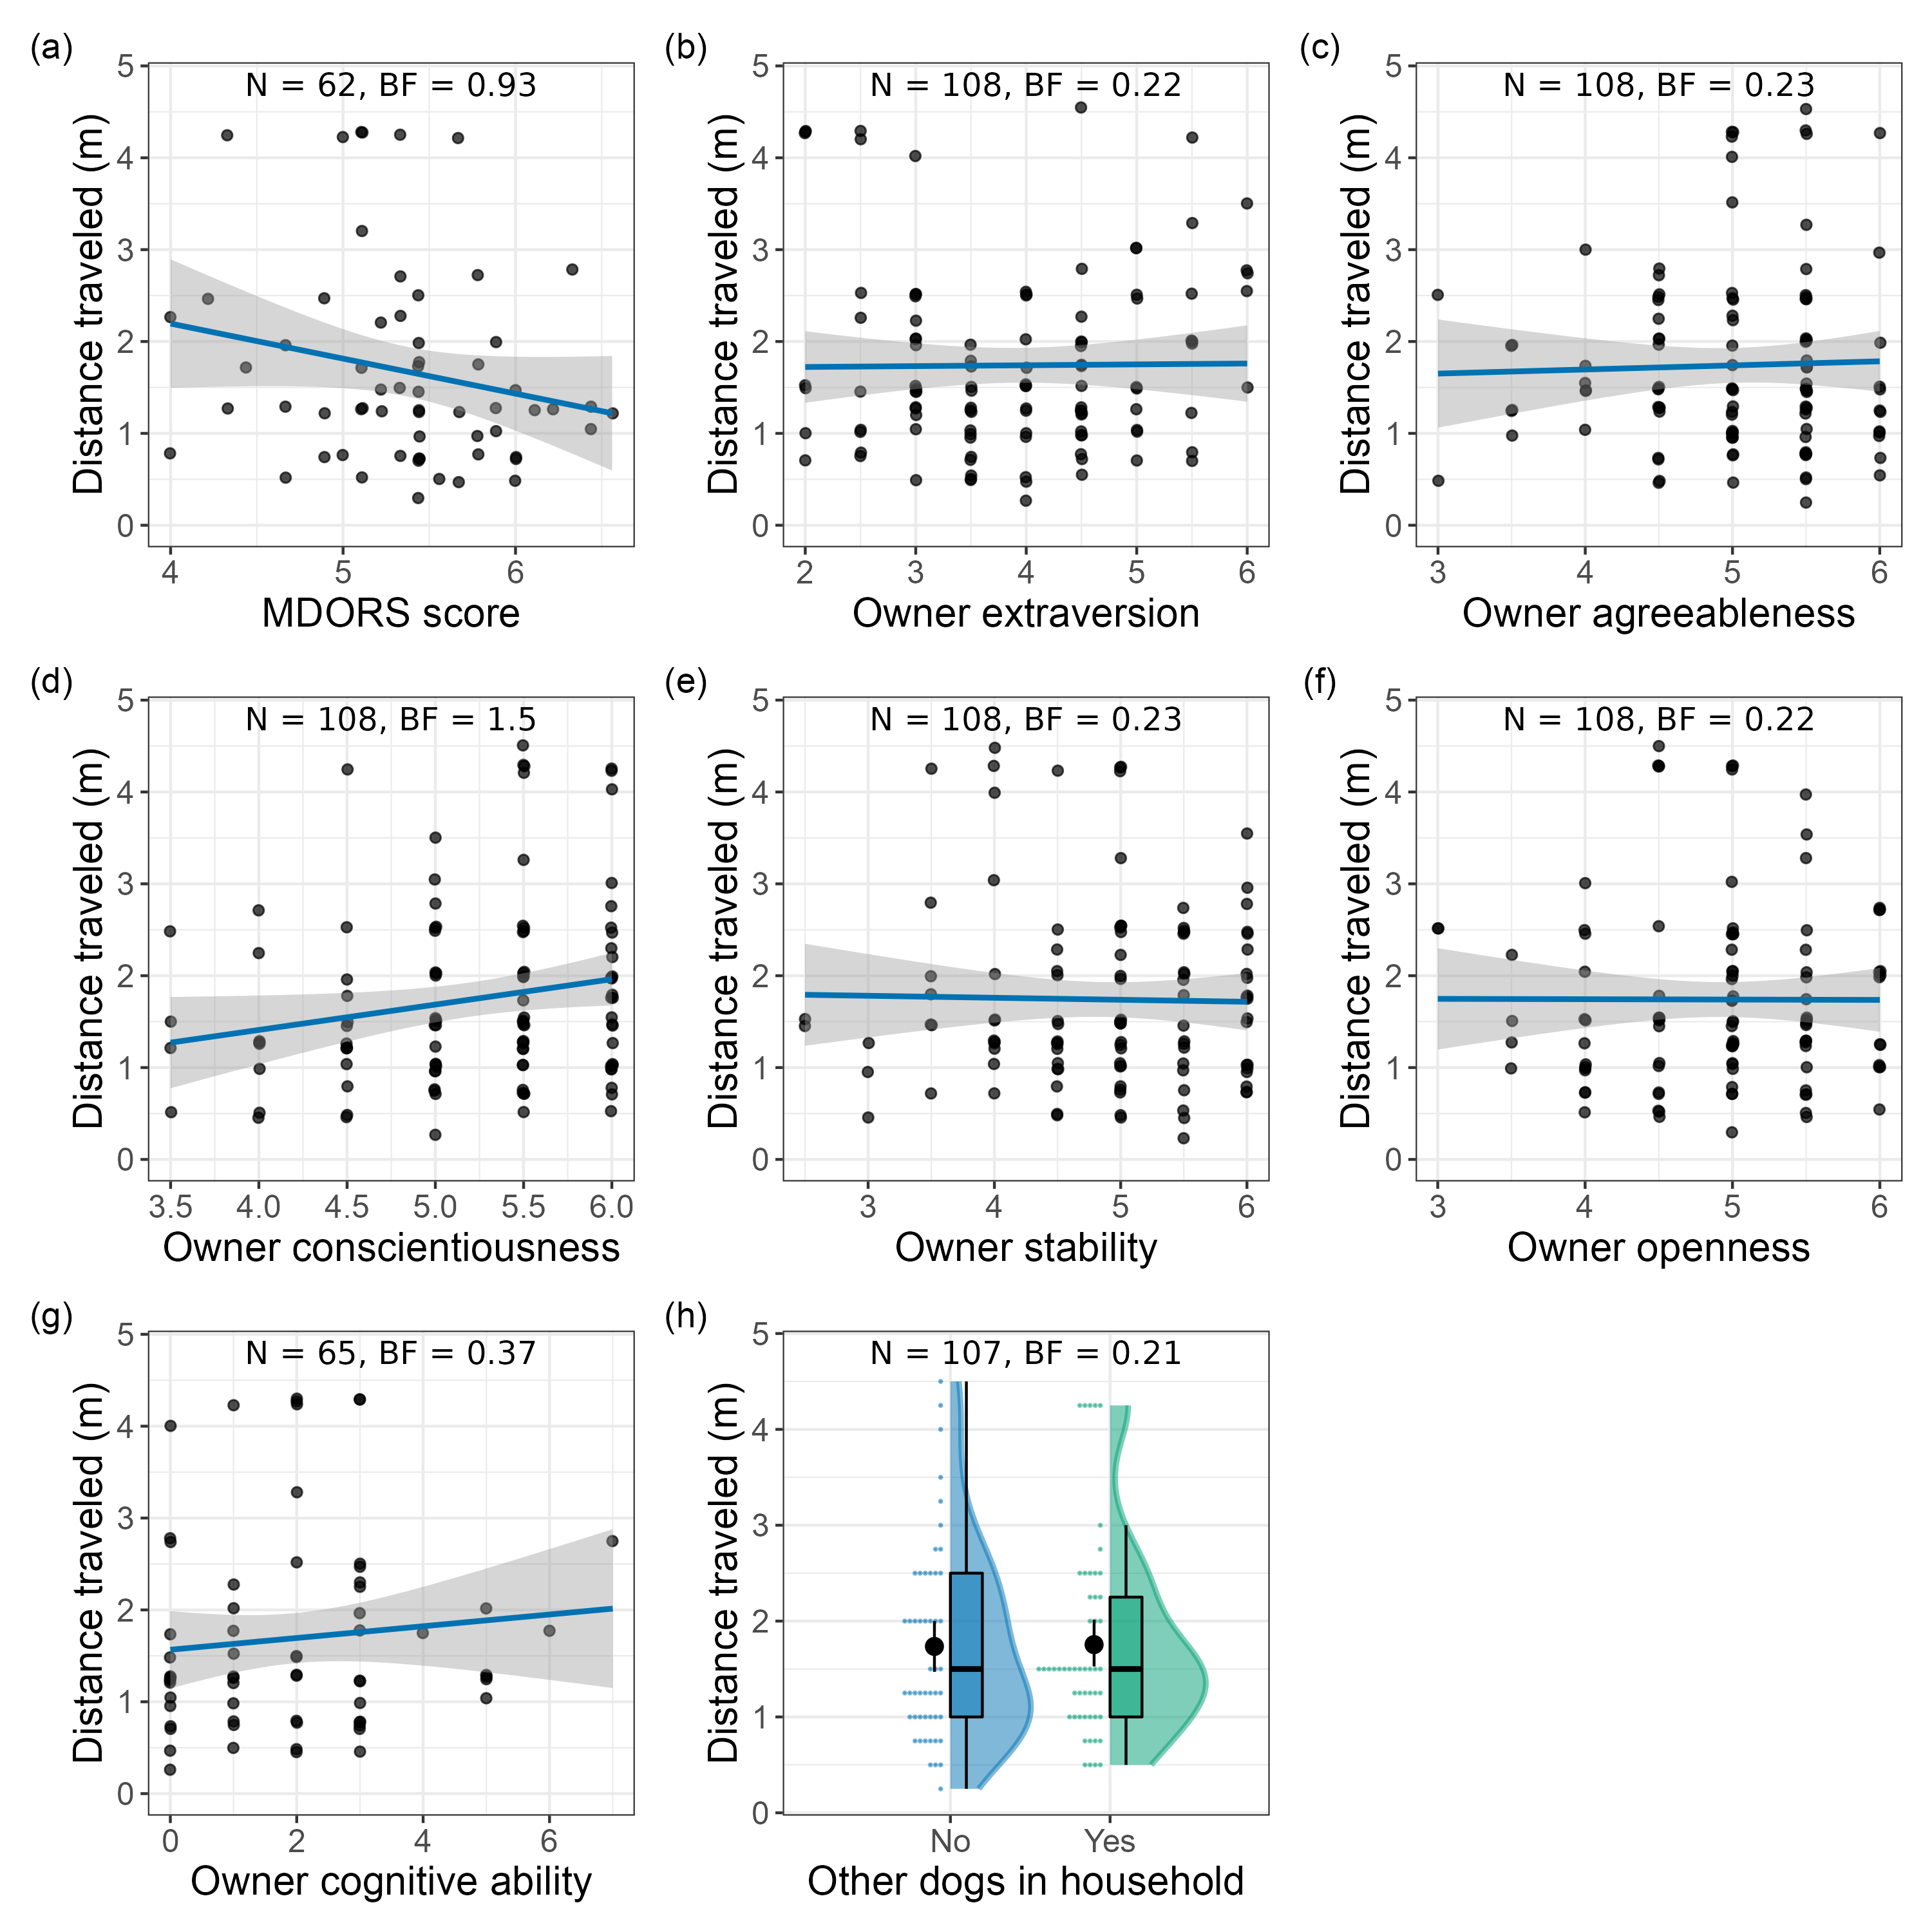
\includegraphics[width=0.95\linewidth]{figures/owner_characteristics} 

}

\caption{Relationship between distance travelled and owner characteristics. Distance traveled was not related to dog (a) Monash Dog Owner Relationship Score, (b-f) owner personality, (g) owner cognitive ability, or (h) whether owners had other dogs in the household. For correlations, dots represent individual dog data points, lines represent best fitting linear regression models, and bands represent 95\% confidence intervals around the regression models. For group comparisons, dots represent individual dog data points, filled shapes represent density distributions, filled dots and error bars represent means and 95\% confidence intervals, boxes represent interquartile ranges, lines within boxes represent medians, and whiskers represent 1.5 times the interquartile range.  Figure used with permission under a CC-BY4.0 license: Stevens et al. (2022); available at https://doi.org/10.31234/osf.io/hyvdq.}\label{fig:owner-char}
\end{figure*}


\end{document}
